%\cleardoublepage
\section{Listening Experiment}
\label{sec:listening-experiment}
%
We aim at investigating, if audio content treated with a constant phase
shift filter can be perceptually discriminated from the original signals.
%
This section discusses the design, procedure and analysis of the
conducted listening experiment, related to this question.
%
%
%
\subsection{ABX Test Framework}
The discrimination performance was tested with the highly sensitive two alternatives,
forced choice ABX test.
%
Stimuli A and X were both randomly assigned to either the reference (original)
or the treatment (phase shift), subsequently ensuring that B contains the other
stimulus than A.
%
According to the ABX test paradigm, test subjects were asked to assign either
X=A or X=B after thorough, non-time-limited comparison of A, B and X.
%
\NewL No looped playback or instantaneous stimulus switching with crossfade or
fast fade-out/fade-in could be utilized, since treatment detection would have become
a trivial task based on the resulting artifacts (i.e. clicks for fade-out/in,
phasing for crossfade).
%
Instead, the stimuli---always (re)-started from the beginning---%
had to be manually started and stopped by the test subjects.
%
This ensures artifact free playback, although with higher interaction.
%
Moreover, the requirements led to some modifications of the utilized webMUSHRA
test framework \cite{Schoeffler2018}, which by default intends seamless switching
and looping by fading out/in.
%
%
%
\subsection{Audio Content}
The 4 monaural audio contents
\begin{itemize}
\item three square wave burst signals, each: 50 Hz, 200 ms on including
40 ms $\sin^2$-fade in and out,  300 ms off.
Fourier series synthesis of the
harmonics $1, 3,\dots, 19$, modal windowing (Kaiser, $\beta=4$) of the Fourier
coefficients. total length 1.5 s @ 120 bpm, periodicity assumed~/~DFT filtering
\item pink noise\footnote{generated by Voss-McCartney algorithm:\\\url{https://github.com/AllenDowney/ThinkDSP/blob/master/code/voss.ipynb}},
lowpass filtered
(4th order Butterworth, cut frequency 300 Hz),
length 2.35 s, non-periodicity assumed~/~FIR filtering
\item castanets\footnote{anechoic version of EBU SQAM CD track 27:\\\url{https://iaem.at/Members/frank/sounds/castanets-dry} },
length 2 s, periodicity assumed~/~DFT filtering
\item Hotel California, Eagles, Hell freezes over, 1994, Geffen,
stereo version mixdown to mono, time range 0:44.938 - 0:48.142, non-periodicity assumed~/~FIR filtering
\end{itemize}
were chosen to create the 5 treatments
\begin{enumerate}[I]
\item square wave burst with $\varphi=-90\degree$
\item square wave burst with $\varphi=-45\degree$
\item lowpass filtered pink noise with $\varphi=-90\degree$
\item castanets with $\varphi=-90\degree$
\item Hotel California with $\varphi=-90\degree$,
\end{enumerate}
%
according to the following considerations:
It is known that human hearing is sensitive to group delay variations of low
frequency square wave bursts \cite{Suzuki1980}, which is assumed to hold for
constant phase shifts as well.
%
To evaluate a potential detection of phase shifts for highly transient audio
material and to check for potential detection of pre-/postringing
due to filtering of such, castanets were included.
%
Phase alignment in noise signals is highly random.
It was assumed that human hearing is sensitive to a varied phase structure of
noise with a low frequency spectrum.
%
Furthermore, a musical record with a percussion sequence---%
commonly considered as very high fidelity production (mixing: E. Scheiner,
mastering: T. Jensen)---was included.
For that content, it was assumed that a constant phase shift might be audible
in the decay of the drumheads or/and in the transients.
%
\NewL For the treatments I, II and IV signal periodicity is assumed and thus
the ideal phase shift filter via DFT (Sec. \ref{sec:periodic-signals}) was
applied.
%
To create treatments V and III, no signal periodicity was assumed for the
whole musical piece as well as for the generated pink noise raw material of 6 minutes
duration.
%
Thus FIR filtering according to Sec.~\ref{sec:aperiodic-signals} was realized.
%
Considering the audio contents as rectangularly windowed signals of infinite
duration, the filter order of 3\,963\,530 ($\approx 90\,\text{s}$!) ensures
that linear convolution of the chosen excerpt of Hotel California is complete.
%
The resulting magnitude ripple of the Blackman windowed FIR is negligible
for the relevant reproduction bandwidth.
%
Since the pink noise length can be arbitrarily set, the same FIR filter was utilized
for consistence.
%
%
%
\subsubsection{Crest Factor Discussion}
%
\begin{figure}[t]
\centering
\includegraphics[width=0.5\textwidth]{graphics/crest-factor}
\caption{Crest factor over phase shift for the 4 audio contents used in the
listening test.}
\label{fig:crestfactor}
\end{figure}
%
An ideal constant phase shifter does not alter the
spectrum of the input signal, nor does it introduce any group delay.
One noticeable technical change concerns the waveform, quantifiable in terms of
the crest factor (CF),
\begin{align}
\CF = 20 \log_{10}\left(\frac{\abs{s}_{\text{PEAK}}}{s_{\text{RMS}}}\right)\quad \text{in dB}.
\label{eq:crestfactor}
\end{align}
During the preparation of this study,
it was speculated that an increase or decrease of the CF
might lead to detectable cues (if there are any) for a phase shift.
%
\NewL Figure~\ref{fig:crestfactor} depicts the CF of the chosen audio contents
for varying phase shifts $\varphi \in [-180\degree, 180\degree]$.
For aperiodic signals (pink noise and Hotel California),
the phase shift is applied to the entire piece
but the CF is evaluated only for the selected part
which is used in the listening experiment.
Notice that the CF is $180\degree$-periodic.
This is because a phase shift of $180\degree$ reverses the polarity of the signal
and the CF remains unchanged.
Among other stimuli, the square wave burst shows the highest variation
of approximately $7$~dB.
Note, however, that due to the silence between the bursts
and the temporal shaping by the fade-in/-out window,
the CF deviates from that of a continuous square wave
(which is theoretically $\CF\!=\!0$~dB for $\varphi\!=\!0\degree, \pm180\degree$
and $\CF\!=\!\infty$ for $\varphi\!=\!\pm 90\degree$).
The CF of castanets is about $15$ to $25$~dB higher than other stimuli
because of its fast attack/decay, very short sustain,
and relatively long silence.
%
\NewL As mentioned in Sec.~\ref{sec:introduction},
phase angles of $-90\degree$ and $-45\degree$ are particularly of our interest
due to the relation with the equalization filter in WFS.
Except for square waves, a phase shift of $-45\degree$ is barely detectable
for most of the audio materials that was tested in informal listening.
Therefore, $-90\degree$ is predominantly tested in this study
whereas $-45\degree$ is included only for square wave bursts.
In Fig.~\ref{fig:crestfactor}, the CF change of the phase shifted stimuli
relative to the original signal ($\varphi=0\degree$) is annotated
above the filled circles \cflabel.

%the technical change of the signal between original and phase-shifted version
%--- i.e. change from low to high crest factor or vice versa ---
%is largest for the chosen audio material assuming a perceptual correlation.
%
%
%
\subsubsection{Audio Signal Processing and Rendering}
%
Each reference audio content (except castanets) was loudness
calibrated to -23 LUFS \cite{ITU1770}.
The according calibration gain was also applied to the associated phase shifted
stimuli.
%
Since the loudness measure of \cite{ITU1770} is suboptimal for castanets,
perceptually motivated re-calibration to -35 LUFS was pursued in order to better
match playback level with the other audio contents.
%
Non-dithered 24~Bit, 44.1~kHz PCM wav-files were rendered for all required stimuli,
carefully monitoring that amplitude clipping---as undesired artifact blended with
the phase shift---does not occur.
%
%
%
\subsection{ABX Test Statistics Considerations}
All test subjects were to rate the 5 different treatments created from the 4
audio contents in mixed, randomized order and---except for the two lead authors---%
without preliminary training or other preconditioning with respect to the research
question.
%
\NewL For each of the 5 treatments 25 ABX trials had to be rated, resulting
in $5\cdot 25=125$ judgments per test subject aiming at evaluation of
individual detection rates in the first instance.
%
Thus, with underlying Binomial distribution model
\cite{Howell2013, faul2007}, these quantities originate from
intended one-side tail hypothesis testing of the $\Hnull(p_\text{detect}=0.5)$
using Bonferroni correction to a target
rejection level $\alpha=0.05$, a target test power $1-\beta=0.95$ and an
effect size of $g=0.4$, which was determined from
preliminary test results using square wave bursts, achieving detection
probabilities of about $p_\text{detect}=0.9$.
%
\NewL Assuming independence of all collected ratings, contingency tables of
detection frequencies can be statistically evaluated with underlying Chi-Square
($\chi^2$) distribution model as post hoc tests.
%
%
%
\subsection{Experiment Procedure}
The listening test was conducted in our loudspeaker array lab with 0.3~s mean RT60
and about $40~\text{dB(A)}_\text{Leq}$
sound pressure level (SPL) of background noise.
%
A large monitor, a keyboard and a mouse were set up on a table, where test subjects
took seat in the middle of the lab during the experiment.
%
The browser based ABX GUI of the webMUSHRA software was hosted on an Apple Mac Mini
connected to an RME Fireface UC.
%
\NewL Playback was presented diotic (i.e. same signal for both ears) using
an electrodynamic, circumaural, open headphone Sennheiser HD 800.
%
Playback level was settled such that for a mono pink noise signal with
$-23~\text{LUFS}$ loudness
(%$-8.2~\text{dB}$ sample peak,
$-7.8~\text{dB}_\text{TruePeak}$,
$-21.3~\text{dB}_\text{RMS}$, i.e.
$13.5~\text{dB}_\text{CF}$)
sound pressure levels (SPLs) of
$72.7~\text{dB(A)}_\text{Leq}$ / $87.7~\text{dB(C)}_\text{Peak}$
were measured for the left and the right channel using a G.R.A.S.
headphone-to-ear coupler and a calibrated Br\"uel \& Kjaer SPL meter according
to the IEC 60318 standard.
%
\NewL 12 test subjects (4 female, 8 male) took part in the listening experiment.
Except one light tinnitus afflicted, all others reported normal hearing.
%
Test subjects' age distribution is given as $\mu_a=29.8$, $\sigma_a=6.5$ years with the
percentiles $a_{0.05}=22.6,~a_{0.25}=25,~a_{0.5}=28,~a_{0.75}=32,~a_{0.95}=40.5$ years.
%
About half of the listening test panel consists of
music production experts and (future) professional musicians
(classical instrument students).
%
The other half recruits from research related, untrained listeners,
occasionally without prior experience in performing listening tests.
%
\NewL For familiarization of the specific ABX GUI, ratings on
full band pink noise with 1~dB level difference were performed by each
test subject prior to the actual listening test.
%
This procedure was accompanied by written operational instructions and remarks,
indicating that the differences to be detected in the actual listening test might be
very subtle and will potentially differ in character compared to that of the training
session.
%
Participants (except the two authors) were left completely uninformed
with respect to the signal manipulation method, thus expecting unbiased
strategies for the detection of differences.
%
\NewL After many pre-listening experiments, we decided against playback of all
25 trials per each treatment in one sequence.
This regularly resulted in an extremely tedious task, that should only be
considered for few well trained and extraordinary performing test subjects.
%
Since, in the first instance, we intended to find effect sizes $g$ for a rather
untrained, non-preconditioned test panel, we set up playback for a mixed
randomized sequence of all 125 trials, divided in 4 parts
(35 + 3 $\cdot$ 30) with longer intermissions.
%
Thus, the results to be presented in the next section, should be
considered for this conditioning.
%
%
%
\subsection{Results}
\subsubsection{Tests on Binomial Distribution}
%
\begin{figure}[t]
\centering
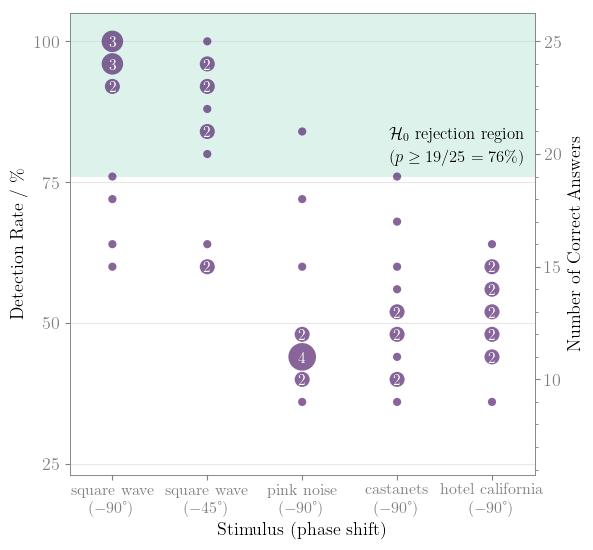
\includegraphics[width=0.5\textwidth]{graphics/scatter}
\caption{Detection rates in percent and number of
correct detections of all test panelists. Small dots without numbering indicate
a performance of a single test subject, whereas increasing dots with numbering
indicate same performance for multiple test subjects. Results within the
\colorbox{colhnull}{shaded area} indicate that guessing is unlikely with statistical significance.}
\label{fig:scatter}
\end{figure}
%
The detection rates (correct discrimination between original and phase shifted
version) of all test subjects for all treatments are shown as a scatter plot in
Fig.~\ref{fig:scatter}.
%
For the $-90\degree$ phase shifted square wave burst, except of three subjects, all
other perform with very high, statistically significant detection rates between
$76\%$ and $100\%$.
%
For the $-45\degree$ phase shifted square wave burst, except of the same  three subjects,
all other show very high, statistically significant detection rates between
$80\%$ and $100\%$.
%
\NewL The $-90\degree$ phase shifted pink noise treatment exhibits only one result
for which guessing can be excluded by statistical significance.
This was produced by one of the preconditioned, trained authors.
%
The majority of detection is slightly below guessing.
%
About the same situation, however with larger spread of the rates, can be observed
for the $-90\degree$ phase shifted castanets treatment.
The one statistically significant result was achieved by another trained,
preconditioned author.
%
All other detection rates fail to reject that guessing took place.
%
\NewL For the musical content, i.e. the percussion sequence in Hotel California,
no statistical significance can be reported.
%
Detection rates spread around the guessing rate ranging from $36\%$ to
$64\%$.

\subsubsection{Tests on Chi-Square Distribution}
The $\Hnull$~(correct and incorrect discrimination occur with equal
frequency) is tested with the $\chi^2$ test per treatment considering all judgments.
%
Bonferroni correction for total of 5 treatments to a target
$\alpha=0.05$ was considered.
%
The results indicate that this $\Hnull$ can be rejected
with very high statistical significance for the two square wave bursts,
but not for the other three treatments.
%
\NewL The $\Hnull$ (detection performance of two treatments is independent)
is tested with the $\chi^2$ test of the contingency table built from two treatments
considering all judgments.
%
Bonferroni correction for the 10 possible pairwise comparisons to a target
$\alpha=0.05$ was considered.
%
The results indicate that this $\Hnull$ can be rejected for
the pairs I vs.~III, IV, V and II vs.~III, IV, V with very high statistical
significance and odds ratios (ORs) between $4.5$ to $6.5$.
%
For the pairs I vs.~II and III vs.~IV, V and IV vs.~V we fail to reject this
$\Hnull$.
For pairwise comparison I vs.~II the $\text{OR}\approx 1.4$ indicates a very small
(however statistically not significant, $p=0.17$) tendency for a different performance.
%
For the other pairs $\text{OR}\approx 1$ indicates very comparable rating performance.
%
%
%
\subsubsection{Rating Durations}
Test subjects took between 70 and 120 minutes in total for the whole listening
experiment, including intermissions.
%
One test subject asked to split the test onto two days for improved power of
concentration.
%
\NewL The webMUSHRA software captures data for rating durations of all trials.
%
This duration is defined as the time interval from initiating the GUI for the
actual trial up to submitting the result and moving on with the next trial.
%
Thus, this duration measure includes all (potentially longer) individual
intermissions of a test subject.
%
Pure playback duration of A,~B,~X per trial,
which is considered a more useful measure, is unfortunately not available.
%
We thus report the percentiles in Table~\ref{tbl:duration} over all rating
durations $t$ in seconds without further statistic evaluation.
%
However, the table easily reveals that the median and the interquartile range---%
that should not overly affected by longer intermission intervals---%
increase following the treatment sequence I to V.
%
\begin{table}[h]
\centering
  \begin{tabular}{ l | c | c | c | c | c}
    %\hline
    treatment &  $t_{0.05} / s$ & $t_{0.25} / s$ & $t_{0.5} / s$ & $t_{0.75}/s$ & $t_{0.95}/s$\\ \hline
    I sq -90 &8.1& 12.4& 17.7& 29.2& 60.9\\ \hline
    II sq -45 &8.9& 15.3& 23.1& 39.8& 95.2\\ \hline
    III pn -90 &13.7& 19.8& 28.7& 47.4& 98.6\\ \hline
    IV cas -90 &11.5 &20.2 &30.0 &48.2 &109.7\\ \hline
    V hc -90 &12.6  &24.4 &35.9 &52.5 &104.2\\ \hline
  \end{tabular}
\caption{Percentiles of the rating duration per ABX trial.}
\label{tbl:duration}
\end{table}


\subsubsection{Qualitative Statements}
Test subjects were asked for handwritten qualitative statements (e.g. detection cues,
artifacts) during the listening experiment.
%
Since this was handled as unforced add-on not all panelists reported back.
%
However, the received statements are highly valuable and can be summarized as follows.
%
\NewL Treatments using square wave bursts were comparably very easy to detect, and
comparing both square waves, the $-90\degree$ treatment was much easier to detect than the
one with $-45\degree$.
%
Most often pitch shifts were used as cues, but also changes in envelopment and
dispersion were reported.
%
\NewL The detection of pink noise treatments was reported as very demanding.
%
Here test subjects indicated changed pitch, roughness, sharpness, subbass
structure, melody and ambience as cues.
%
For castanets test subjects reported a hard time for detection and admitted
pure guessing very often
using either the pitch or/and the characteristics of the very first transient
(change of attack, punch and crispness)
to discriminate treatment and reference.
%
No pre-/postringing artifacts were stated for the castanets.
%
%The test subject linked to the significant detection result explicitly excluded
%this as an occurring artifact on request.
%
\NewL For the percussion sequence (Hotel California) most reports agreed on pure guessing.
%
However, test subjects also reported there to use changed decay of drumheads and
changed pitch as cues as well as smeared transients.
%
\NewL One test subject reported that A,B and X were perceived with different pitches
for the square wave bursts.
%
Here, due to the forced choice design, the achieved detection rates
must fail to reject $\Hnull$, which was confirmed post-hoc.
